\chapter{Machine Learning}
El \textbf{Machine Learning} es un campo dentro de la ciencia de datos que se centra en la creación y entrenamiento de modelos de predicción con el objetivo de minimizar el error de salida ante una nueva entrada que el modelo no ha usado en la fase de entrenamiento.

El \textbf{Machine Learning} (aprendizaje automático) es un campo de la Inteligencia Artificial que se centra en el desarrollo de técnicas que permitan a las computadores extraer conocimiento a partir de unos datos.\\
\linebreak
Estos datos pueden estar definidos de una gran número de formas, observaciones recogidas por sensores, imágenes, valoraciones de usuarios, etc. En el caso particular de este trabajo en el que se enfoca este proyecto, el \textbf{conjunto de datos} con el que se va a trabajar tiene una cantidad de \textbf{muestras} en la que cada muestra tiene un número fijo de \textbf{características} que identifican a cada muestra. Además, el conjunto de datos con el que se está trabajando, contiene una serie de \textbf{etiquetas} asignada a cada muestra.\\
\linebreak
\section{Tipos de problemas}
En esta sección se van a exponer algunos de los distintos tipos de problemas que podemos encontrarnos, agrupándolos siguiendo ciertos criterios. Como cualquier otro problema, existen una gran cantidad de criterios distintos que se pueden usar para clasificar el problema, en esta sección se han usado los criterios en función de los datos disponible ó en función de la tarea que se quiere conseguir.
\subsection{Agrupamiento en función de los datos disponibles}
Se puede usar la naturaleza de los datos para definir varios tipos de algoritmos, ya que la metodología a seguir cuando se trabaja con datos \textbf{etiquetados} o con datos sin etiquetar es distinta. Usando esta idea, las técnicas usadas en ML pueden ser agrupadas en \textbf{aprendizaje supervisado}, \textbf{no supervisado} ó \textbf{semi-supervisado}:
\begin{itemize}
	\item \textbf{Aprendizaje supervisado:} Este conjunto de técnicas se caracteriza debido a que cada muestra tiene una ó más \textbf{etiquetas}(variable/s objetivo) y tiene como finalidad hacer uso de las características de cada muestra para \textbf{predecir} las variables objetivo de nuevas muestras que no pertenecen al conjunto de datos inicial. Alguna de las tareas que entran dentro de este grupo son \textbf{Clasificación} ó \textbf{Regresión}
	\item \textbf{Aprendizaje no supervisado:} A diferencia del anterior, las técnicas de aprendizaje no supervisado se diferencian en que las muestras \textbf{no están etiquetadas}, por lo que no se puede \textbf{predecir} ninguna variable. Estas técnicas se caracterizan por ser capaces de \textbf{reconocer patrones} dentro del conjunto de datos, etiquetando las nuevas entradas haciendo uso de ellos. La tarea más común es \textbf{Clustering}
\end{itemize}
Anteriormente se han mencionado tareas como \textbf{clasificación}, \textbf{regresión} o \textbf{clustering}, en la siguiente sección se va a profundizar más, explicando en que consiste cada una y que objetivos tienen.
\subsection{Agrupamiento en función de la tarea}
\begin{itemize}
	\item \textbf{Clasificación:} Como se mencionó previamente, esta tarea tiene sentido cuando se usa un conjunto de datos que está etiquetado. El objetivo principal de clasificación consiste en dada una nueva muestra, \textbf{predecir} una o varias etiquetas en función del conjunto de datos que se ha usado. Estas etiquetas suelen ser variables \textbf{discretas}
	\item \textbf{Regresión:} A diferencia de clasificación, donde las variables objetivo son discretas, en este caso las variables objetivo son continuas. El propósito de estas técnicas es el de predecir un \textbf{valor} para nuevas muestras.
	\item \textbf{Clustering:} El objetivo es el de detección de patrones usando datos no etiquetados.
\end{itemize}
Dentro de las tareas de clasificación, se pueden dividir en varios grupos. En la siguiente sección se va a explicar los distintos tipos de clasificación, ya que ayudara a entender la naturaleza del problema que se esta tratando en este trabajo.
\section{Tipos de clasificación}
Como ya se ha mencionado previamente, clasificación usa un conjunto de datos para predecir un valor de una o mas variables de salida. Este tipo de problema puede clasificarse siguiendo muchos criterios, pero en nuestro caso, el criterio que se ha considerado más interesante en función del problema que se esta solucionando es usar el \textbf{tipo de variable} que se va a predecir. Siguiendo este criterio, se pueden encontrar clasificación binaria, multi-clase, multi-etiqueta y multi-dimensional.
\subsection*{Clasificación binaria}
Este es el tipo de clasificación más sencilla, ya que la variable objetivo solo va a tener dos posibles valores. Estos valores se conocen como clase positiva (1) ó clase negativa (0). De aquí viene el nombre de clasificación \textbf{binaria}, ya que la variable objetivo es binaria.\\
Ejemplos de este tipo de clasificación son detectar si un mensaje es spam, si en función de ciertos valores una bomba de agua puede fallar, o detectar si un cliente de un banco va a tener deudas usando ciertos parámetros.
\begin{figure}[H]
	\centering
	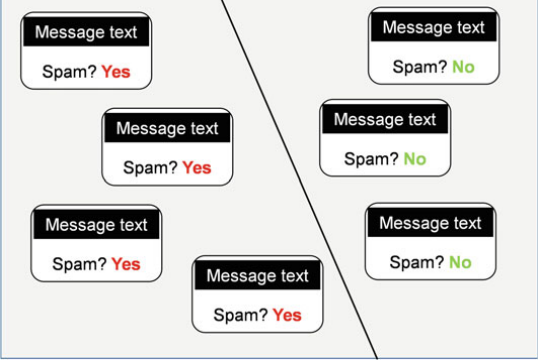
\includegraphics[scale=0.4]{binary-class.png}
	\caption{Ejemplo de clasificación binaria}
	\label{fig:bclass}
\end{figure}
En la Figura \ref{fig:bclass} se puede observar un problema de clasificación binaria, donde se quiere identificar si un correo es spam o no. 
\subsection*{Clasificación multi-clase}
Los conjuntos de datos que se usan en clasificación multi-clase son una generalización del caso de clasificación binaria. Solo existe una única variable objetivo, siendo la principal diferencia que esta puede tener cualquier valor dentro de un conjunto valores. Es importante destacar que estos valores son \textbf{discretos} y \textbf{finitos}.
\begin{figure}[H]
	\centering
	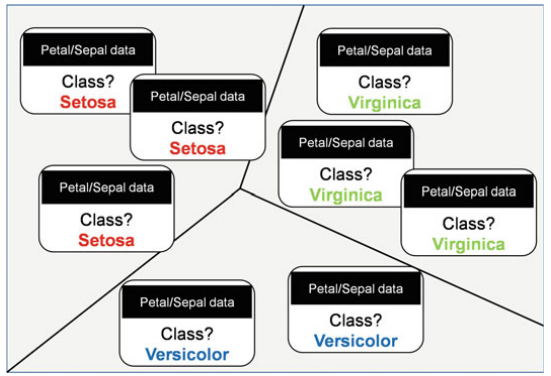
\includegraphics[scale=0.4]{multiclass-class.png}
	\caption{Ejemplo de clasificación multi-clase: Clasificación de la flor del Iris}
	\label{fig:mcclass}
\end{figure}
La Figura \ref{fig:mcclass} representa el que es quizás el ejemplo más conocido de este tipo de clasificación: la \textbf{clasificación de la flor del Iris}, donde en función de la longitud y anchura del sépalo y del pétalo, se predice si la flor es setosa, virgínica o versicolor.\\\\
\linebreak
Muchos de los algoritmos que se usan en Aprendizaje Automático han sido diseñados para clasificación binaria. Con el objetivo de adaptar estos algoritmos existentes a este tipo de problema, existe una técnica llama \textbf{binarización de clase}.
Dos de los enfoques más usados en la actualidad son \textbf{OVA} (\textit{one vs all}) y \textbf{OVO} (\textit{one vs one}). Ambos enfoques tratan de dividir el problema de clasificación multi-clase en varios problemas de clasificación binaria. La diferencia reside en la manera de dividir el problema:
\subsubsection*{One VS All}
Por cada clase, se entrena un clasificador binario donde todas las muestras que pertenecen a la clase seleccionada se selecciona como la clase positiva, el resto como la clase negativa. Una vez que se quiere predecir una nueva muestra, por cada modelo entrenado, se obtiene la probabilidad de que pertenezca a la clase positiva, seleccionando como clase predicha aquella con mayor probabilidad.
\begin{figure}[H]
	\centering
	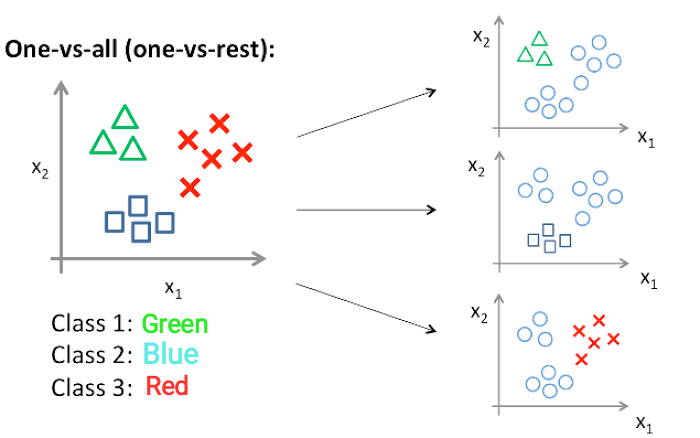
\includegraphics[scale=0.4]{ova.png}
	\caption{Ejemplo de One vs All}
	\label{fig:ova}
\end{figure}
Se puede ver un claro ejemplo de esta enfoque en la Figura \ref{fig:ova}. En este caso se escogería de todo el conjunto de datos una clase, y se clasifica contra el resto de clases que forman el problema, obteniendo así un problema de tipo binario.
\subsubsection*{One VS One}
A diferencia de \textit{OVA}, por cada par distinto de clases, se entrena un clasificador binario usando una como positiva y otra como negativa. Una vez que llega una nueva muestra, se elige por votación la clase predicha.
\begin{figure}[H]
	\centering
	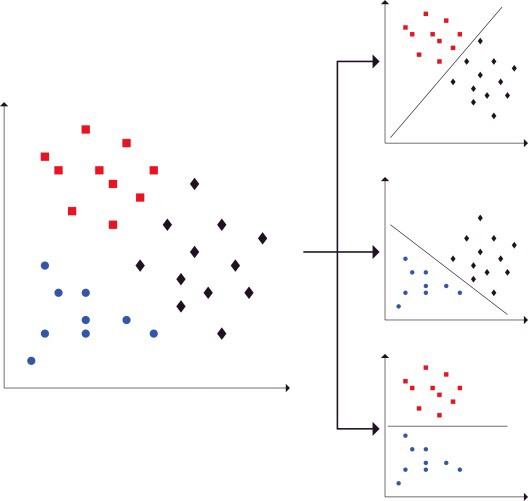
\includegraphics[scale=0.4]{ovo}
	\caption{Ejemplo de One vs One}
	\label{fig:ovo}
\end{figure}
En la Figura \ref{fig:ovo} se aprecia como dado el conjunto de datos, por cada par de clases (rojo-negro, negro-azul, rojo-azul), se entrena un clasificador binario, pudiendo así identificar a que clase pertenecería una muestra que no forme el conjunto de datos original.
\subsection{Clasificación ordinal}
\label{sec:ord_class}
Clasificación ordinal es un caso particular de clasificación multi-clase donde existe una relación de orden entre las clases.\\
Un ejemplo de este tipo de clasificación es el de predecir la valoración de una película, predecir las preferencias de una persona (en desacuerdo, de acuerdo).\\
\linebreak
La propuesta explicada en el articulo \textit{A Simple Approach to Ordinal Classification} es la siguiente:\\
\linebreak
En lugar de clasificar $k$ clases, se van a entrenar $k-1$ clasificadores binarios donde la variable objetivo del modelo $M_i$ representa la \textbf{probabilidad} de que la clase sea mayor (según el orden) que la clase $K_i$. El siguiente ejemplo ayuda a explicar este enfoque:\\
\linebreak
Se quiere predecir el ranking (de 1 a 5) que un usuario le va a dar a una película. Para ello se van a entrenar los siguientes $4$ modelos:
\begin{enumerate}
	\item El primer modelo calcula la probabilidad de que el ranking predicho sea mayor que 1.
	\item El segundo modelo calcula la probabilidad de que el ranking predicho sea mayor que 2.
	\item El tercer modelo calcula la probabilidad de que el ranking predicho sea mayor que 3.
	\item El cuarto modelo calcula la probabilidad de que el ranking predicho sea mayor que 4.
\end{enumerate}
Una vez que se han calculado las probabilidades, el modelo escoge aquella clase con mayor probabilidad. Obviamente, es muy importante optar por este enfoque que el modelo seleccionado sea capaz de obtener la \textbf{probabilidad} de que una muestra pertenezca a una clase. Los modelos seleccionados en este capítulo son capaces de obtener las probabilidades de clase.
\subsection{Clasificación multi-etiqueta}
\label{sec:ml}
A diferencia de los anteriores tipos de clasificación, cada muestra tiene un \textbf{conjunto de variables objetivo} en lugar de una única variable. En este caso, el número de variables objetivo es fijo, siendo estas de tipo binario. A cada combinación distinta de valores se conoce como \textit{labelset}.\\
Los algoritmos que usados para este tipo de problema deben de ser capaces de realizar varias predicciones, ya sea modificando los datos originales o adaptando algoritmos de clasificación binaria o multi-clase.\\
\linebreak
Un ejemplo de este tipo de clasificación puede ser el de comprobar si una imagen contiene ciertos elementos.
\begin{figure}[H]
	\centering
	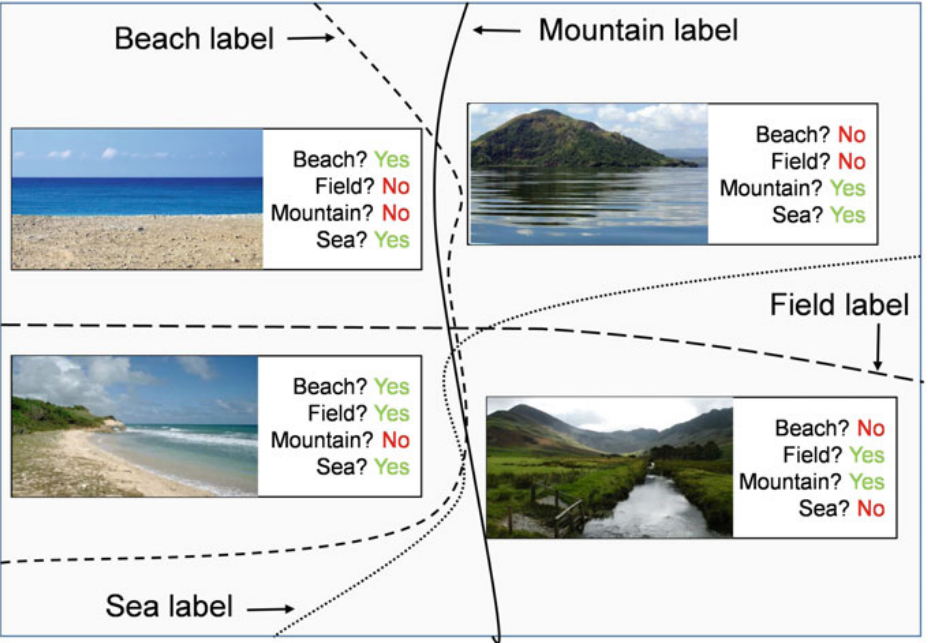
\includegraphics[scale=0.4]{multilabel-class.png}
	\caption{Ejemplo de clasificación multi-etiqueta}
	\label{fig:mlclasss}
\end{figure}
Se puede observar en la Figura \ref{fig:mlclasss} que se está intentando clasificar si un paisaje es playa, campo, montaña o mar. Esta claro que una playa debería de dar positivo tanto en playa como en mar, por lo que en este tipo de problemas hay varias variables objetivo que se quieren predecir.\\
\linebreak
\subsubsection*{Enfoques}
A la hora de clasificar datos con múltiples etiquetas, se ha optado por dos enfoques: \textbf{transformar los datos} y \textbf{adaptar los métodos/algoritmos existentes}. \linebreak
El primero de los enfoques se centra en aplicar técnicas de transformación sobre el conjunto de datos con el que se esta trabajando para obtener así uno o varios conjuntos de datos a los que se les puede aplicar clasificación multi-clase o binaria. \linebreak
El segundo, se centra en modificar los algoritmos de clasificación para que sean capaces de manejar estos conjuntos de datos, produciendo así más de una salida.
\subsubsection*{Transformación del conjunto de datos}
Este tipo de clasificación es una tarea más compleja que la clasificación tradicional, y una de las primeras propuestas para resolver este problema es el de transformar los datos para obtener así uno (o varios) problemas más simples.
Los enfoques que se han propuesto son:
\begin{enumerate}
	\item \textbf{Desplegar las muestras multi-etiqueta} Este enfoque descompone cada instancia en tantas instancias como etiquetas contiene, clonando los atributos asociados a cada muestra. La salida será un problema multi-clase, conteniendo más muestras que el conjunto de datos original.
	\item \textbf{Usar el \textit{labelset} como identificador de clase}: Partimos de la idea de usar cada combinación de \textit{labelset} que se encuentre en el conjunto de datos. De esta manera, se obtiene un conjunto de datos multi-clase con el mismo número de instancias y con tantas clases como combinaciones de labelset se encuentren el conjunto de datos original. Este enfoque también se conoce como \textbf{\textit{Label PowerSet}}.
	\item \textbf{Aplicar técnicas de binarización}: Al igual que para el problema multi-clase, se pueden adaptar estas técnicas. El método más común se llama \textbf{Binary Relevance}. En este enfoque se van a entrenar un clasificador por cada etiqueta, clasificando si la etiqueta asociada es positiva o negativa. 
\end{enumerate}
\subsection{Clasificación multi-dimensional}
Al igual que la clasificación multi-clase es una generalización del caso binario, la clasificación multi-dimensional es una generalización de la clasificación multi-etiqueta.\\
En este caso, cada muestra tiene un conjunto fijo de variables objetivo que pueden tomar cualquier valor dentro de un conjunto de posibles valores.
\pagebreak
\section{Metodología}
En esta sección se va a explicar cuales han sido las distintas fases por las que se ha pasado durante el desarrollo de la solución al problema que se está trabajando.
\subsection{Preprocesamiento}
Esta fase es una de las más importantes a la hora de afrontar un problema de aprendizaje automático.\\
El objetivo principal es el de realizar las transformaciones necesarias sobre el conjunto de datos original para que los modelos seleccionados tengan el mejor rendimiento posible. Las transformaciones más comunes que se suelen aplicar son las siguientes:
\begin{itemize}
	\item \textbf{Codificación de variables categóricas:} Existen algoritmos que solo son capaces de trabajar con variables numéricas. Estas transformaciones se realizan con el objetivo de que estos algoritmos puedan trabajar con estas variables, transformando de categóricas a numéricas.
	\item \textbf{Eliminación de muestras ruidosas:} Puede darse el caso de que existan ciertas muestras que introduzcan errores (ruidos) a la hora de predecir. Detectar estas muestras y eliminarlas puede provocar una mejora en el rendimiento de los modelos.
	\item \textbf{Tratamiento de valores perdidos:} Al igual que existen modelos que no son capaces de funcionar con variables categóricas, existen modelos que no permiten variables con valores perdidos. Existe una gran cantidad de técnicas para inferir estos valores perdidos a partir del resto de conjunto de datos. Otra opción también valida puede ser eliminar la variable con valores perdidos, teniendo en cuenta muy posiblemente se pierda información. Este enfoque se suele usar cuando existen variables que tienen una cantidad muy grande de valores perdidos.
\end{itemize}
\subsection{Conjuntos de entrenamiento y de test}
Uno de los principales retos del aprendizaje automático es el de que los modelos predigan valores nuevos y que no han \quotes{visto} nunca. Para validar si un modelo va a ser capaz de cumplir cuando se pide una predicción sobre una muestra nueva, se suele dividir el conjunto de datos inicial en dos: el conjunto de entrenamiento y el de test.\\
\textbf{El conjunto de entrenamiento}, como su nombre indica, es una parte del conjunto de datos inicial que se va a usar para \textbf{entrenar} el modelo. Se entiende como fase de entrenamiento a los pasos que realiza el modelo sobre los datos para extraer el conocimiento del conjunto de datos.\\
\textbf{El conjunto de test}, va a estar formado también por una parte del conjunto de datos inicial que el modelo \textbf{NO} ha usado durante el entrenamiento. De esta forma, se puede comprobar como se va a comportar el modelo sobre unas muestras nuevas.\\
\linebreak
Esta división es muy importante, ya que ayuda a detectar casos donde el modelo ha sufrido de \textbf{sobre-aprendizaje}. 
\subsubsection*{Sobre-aprendizaje}
Este problema se puede observar si el modelo es capaz de predecir muy bien todas las muestras del conjunto de entrenamiento, pero cuando intenta predecir un conjunto de datos nuevo, no es capaz de predecirlo con la misma eficacia.\\
Esto ocurre cuando el modelo ha aprendido el ruido existente en el conjunto de datos de entrenamiento y el modelo \textbf{espera} que este ruido aparezca también en el conjunto de datos de test. 
\subsection{Conjuntos de validación}
\label{sec:validation}
A la hora de determinar la capacidad de predicción del modelo seleccionado, no basta con definir un conjunto de entrenamiento para entrenar el modelo y un conjunto de test para comprobar el rendimiento con datos que el algoritmo no conoce. Aunque a primera vista esta parece una técnica correcta, tiene varios inconvenientes:
\begin{itemize}
	\item Cuando se ajustan los hiper-parámetros de los modelos, se podría llegar a ajustar el modelo al conjunto de test, produciendo un sobre-ajuste.
	\item Solo se esta usando una parte de los datos para validar el modelo, nada asegura que el conjunto de test sea representativo del conjunto de datos con el que se está trabajando.
\end{itemize}
Para solventar estas y algunos otros problemas que tiene esta metodología, se usa la \textbf{validación cruzada}.\\
\linebreak
En lugar de usar el conjunto de entrenamiento para entrenar un único modelo, se divide el conjunto de entrenamiento en $k$ partes, entrenando $k$ modelos usando $k-1$ subconjunto y el restante como de test. \\
\begin{figure}[H]
	\centering
	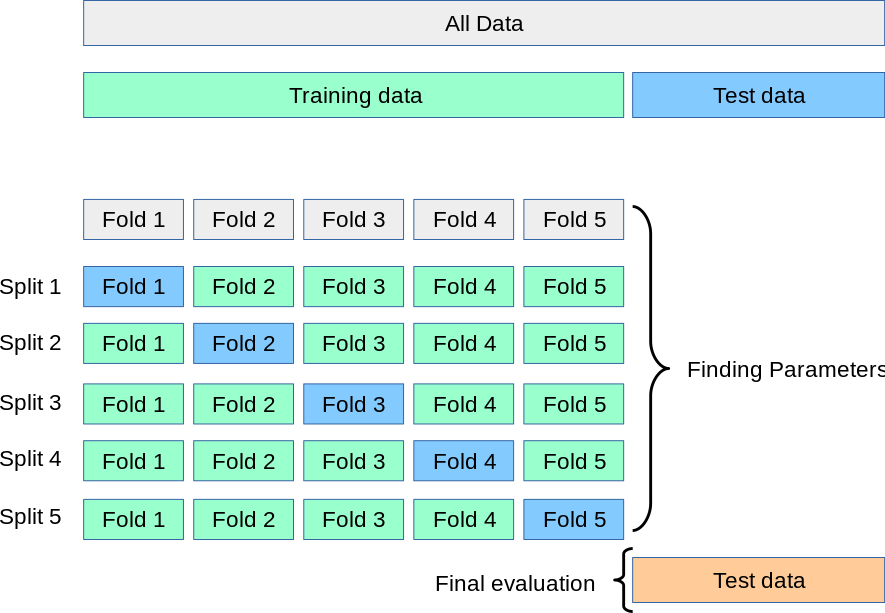
\includegraphics[scale=0.4]{grid_search_cross_validation.png}
	\caption{Ejemplo de validación cruzada con $k=5$}
	\label{fig:cross-validation}
\end{figure}
Como se aprecia en la Figura \ref{fig:cross-validation}, se ha dividido el conjunto de datos en 5 conjuntos (folds), usando en cada iteración 4 para entrenar el modelo y uno para verificar con datos que el modelo no ha visto. Finalmente, se usa el conjunto de test (habiendo entrenado previamente el modelo con todo el conjunto de entrenamiento).
La primera fase del proceso de extracción de conocimiento de un conjunto de datos va a ser precisamente esta, haciendo uso de una serie de modelos, se comprobará el rendimiento y se tomará la decisión de si el conjunto de datos es válido o no. En el caso de que todos los modelos seleccionados no funcionen correctamente, se debería de volver a la fase de recolección de datos, con las indicaciones necesarias para lograr un conjunto inicial lo suficientemente bueno.
\subsection{Análisis de resultados}
En el caso de que los modelos se comporten bien, el siguiente paso a realizar es el de analizar donde flaquean los algoritmos. Una vez detectado los problemas o defectos que tienen los modelos entrenados, se puede realizar un proceso de ajuste sobre los distintos parámetros del modelo.\\
\linebreak
Otra parte importante de este análisis es ver posibles problemas en el conjunto de datos (des-balanceo de clases, valores perdidos, ruido, etc) que está causando un mal comportamiento en el modelo e intentar solventarlos realizando cambios en el conjunto de datos inicial.
\pagebreak
\section{¿Como medir el rendimiento de un modelo?}
Se ha hablado en secciones anteriores sobre el rendimiento de un modelo, pero no se ha mencionado como se puede obtener. Este rendimiento se obtiene usando \textbf{métricas}\\
\linebreak
Antes de explicar que métricas se han usado, es muy importante tener en cuenta el tipo de problema que se está afrontando, ya que las métricas que se usan en clasificación no son validas para problemas de regresión, ya que son problemas muy distintos.
\subsection{Rendimiento de modelos de regresión}
Para comprobar el comportamiento de los distintos modelos seleccionados, se han usado las siguientes \textbf{métricas de regresión}: \textit{\textbf{Coeficiente de determinación}} (se denota como $R^2$), \textit{\textbf{Desviación de Poisson}} y \textit{\textbf{Error cuadrático medio}}
\subsubsection*{Coeficiente de determinación}
Se define como \textbf{coeficiente de determinación} como la proporción de la varianza total explicada por la variables independientes del modelo. Proporciona una indicación de como de bueno es un ajuste y por tanto, una medida de como de bueno es el modelo cuando predice nuevas muestras.\\
\linebreak
Matemáticamente, se define el coeficiente de determinación como:
\[R^2 (y, \hat{y}) = 1 - \frac{\sum_{i=1}^{n}(y_i - \hat{y}_i)^2}    {\sum_{i=1}^{n} (y_i - \overline{y})^2}\]
Donde:
\begin{itemize}
	\item $y$ es el conjunto de valores reales para las variables objetivo.
	\item $\hat{y}$ es el valor predicho para los valores objetivo.
	\item $\hat{y}_i$ es la predicción de la i-ésima muestra.
	\item $y_i$ es el valor real de la i-ésima muestra.
	\item $\overline{y} = \frac{1}{n} \sum_{i=1}^{n} y_i$.
	\item $n$ es el numero de muestras del conjunto.
\end{itemize}
\subsubsection*{Desviación de Poisson}
Esta métrica se calcula como: 
\[
D(y,\hat{y}) = 2\sum_{i=1}^{n}[y_i\log(\frac{y_i}{\hat{y_i}}) - (y_i-\hat{y_i})]
\]
Donde:
\begin{itemize}
	\item $y$ es el conjunto de valores reales para las variables objetivo.
	\item $\hat{y}$ es el valor predicho para los valores objetivo.
	\item $\hat{y}_i$ es la predicción de la i-ésima muestra.
	\item $y_i$ es el valor real de la i-ésima muestra.
	\item $n$ es el numero de muestras del conjunto.
\end{itemize}

\subsubsection*{Error cuadrático medio}
El error cuadrático medio de un estimador mide el promedio de los errores al cuadrado.\\
Matemáticamente, se define el error cuadrático medio como:
\[MSE(y,\hat{y}) = \frac{1}{n} \sum_{i=1}^{n} (y_i - \hat{y}_i) ^2\]
Donde:
\begin{itemize}
	\item $y$ es el conjunto de valores reales para las variables objetivo.
	\item $\hat{y}$ es el valor predicho para los valores objetivo.
	\item $\hat{y}_i$ es la predicción de la i-ésima muestra.
	\item $y_i$ es el valor real de la i-ésima muestra.
	\item $n$ es el numero de muestras del conjunto.
\end{itemize}
\pagebreak
\subsubsection*{Gráficos}
Además del uso de las métricas mencionadas previamente, se han creado las siguientes gráficas para visualizar los errores que esta haciendo un modelo en concreto. Esto ayuda a la toma de decisiones en fases siguientes.\\
Las gráficas que se han desarrollado son las siguientes:
\begin{itemize}
	\item Gráfico de dispersión de errores.
	\item Cantidad de errores por rango. (probablemente sea mejor cambiar este nombre, pero es el nombre que se me ocurrió)
\end{itemize}
El gráfico de dispersión de errores consiste en mostrar en la misma gráfica el valor real de las variables objetivo y el valor predicho por nuestro modelo. Esto nos permite ver como de juntos están las predicciones, identificando así en que zonas el algoritmo se está equivocando más frecuentemente.\\
\begin{figure}[H]
	\centering
	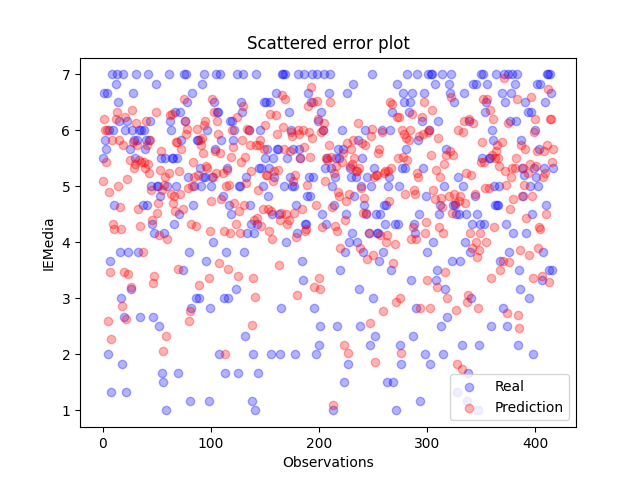
\includegraphics[scale=0.6]{scattered.png}
	\caption{Ejemplo de gráfico de dispersión de errores}
	\label{fig:scattered_example}
\end{figure}
En la Figura \ref{fig:scattered_example} podemos ver un ejemplo real de este tipo de gráficos. En rojo se representan los valores predichos mientras que en azul representa los valores reales. En un caso ideal, los puntos reales y los predichos aparecerían superpuestos, pero en el problema del mundo real predecir el valor exacto es muy complicado, debido a la gran cantidad de variables que pueden formar el problema. En estos casos lo que se busca es que la distancia entre los puntos rojos y los puntos azules estén lo más agrupados posibles.
\pagebreak
El segundo gráfico consiste en lo siguiente:
Los modelos que han sido entrenados están prediciendo valores medios. El proceso seguido para realizar estos gráficos ha sido el de obtener los valores redondeados tanto de la predicción como del valor real. Si el valor redondeado de la predicción y del dato real son distintos, se ha considerado como error. Sumando estos errores, se puede generar un gráfico de barras como el siguiente para tener una visión más clara de en que zonas de la predicción el algoritmo esta funcionando peor:
\linebreak
\begin{figure}[H]
	\centering
	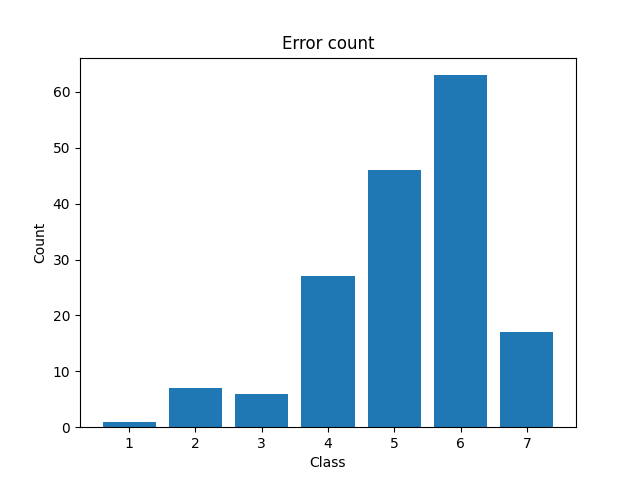
\includegraphics[scale=0.6]{error_hist.png}
	\caption{Ejemplo de gráfico de errores por rango}
	\label{fig:error_hist_example}
\end{figure}
En la Figura \ref{fig:error_hist_example} presenta un ejemplo de este tipo de gráfico. Se puede observar como para valores bajos (de 1 a 3) la cantidad de errores cometidos es menor. Mientras que a medida que estos valores crecen, se aprecia como se ha producido un mayor número de errores.\\
Este gráfico proporciona una idea de para que valores el modelo se ha comportado mejor y para cuales se ha comportado mejor.
\subsection{Rendimiento de modelos de clasificación}
\label{metric:class}
Al igual que en los modelos de regresión, en clasificación se hace uso de métricas para ver el comportamiento de los modelos entrenados. A continuación se explica qué métricas se han usado:
\subsubsection*{Accuracy}
Esta métrica mide el porcentaje de casos que el modelo ha clasificado correctamente.
\[accuracy(y,\hat{y})=\frac{1}{n_{samples}}\sum_{i=1}^{n_{samples}}1(\hat{y_i}=y_i)\]
\subsubsection*{Matriz de confusión}
Cada entrada $i.j$ de la matriz se define como el número de observaciones del grupo $i$ que han sido predichas como del grupo $j$. Un ejemplo de matriz de confusión para el problema que se esta tratando es:
\begin{figure}[H]
	\centering
	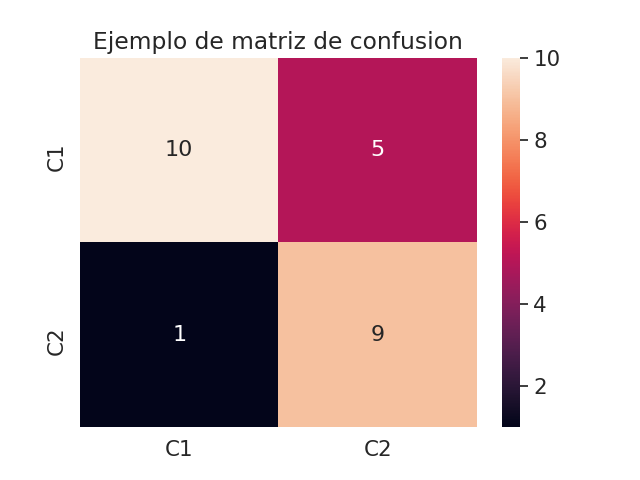
\includegraphics[scale=0.8]{conf_matrix.png}
	\caption{Ejemplo de matriz de confusión}
	\label{fig:conf_matrix}
\end{figure}
En la Figura \ref{fig:conf_matrix} se puede ver cuantas muestras de una clase el modelo predijo como correctas (de la misma clase) y cuantas muestras de una clase predijo como erróneas (de distinta clase).\\
\clearpage
A partir de la matriz de confusión, se pueden sacar las siguiente métricas:
\[Precision = \frac{TP} {TP + FP}\]
\[Recall = \frac{TP}{TP + FN}\]
\[FPR = \frac{FP}{FP + TN}\]
\[F1\_score = 2 \times \frac{Precision \times Recall}{Precision + Recall} \]S
Intuitivamente, \textbf{Precision} mide la habilidad del modelo de no clasificar como \textbf{positiva} una muestra que es \textbf{negativa}, mientras que \textbf{Recall} mide la habilidad del modelo para clasificar bien todas las muestras positivas.\\
\linebreak
Cabe destacar que se han explicado para el caso de clasificación binaria, pero estas métricas se pueden extender para la clasificación multi-clase y multi-etiqueta.
\subsubsection*{Curva ROC y AUC}
Partiendo de lo explicado sobre la matriz de confusión, la curva ROC (Receiver Operating Characteristic Curve) es un gráfico donde se representa el \textbf{FPR} (False Positive Rate) en el eje \textbf{X} y el \textbf{TPR} (True Positive Rate o Recall) en el eje \textbf{Y}. Se escogen estas métricas debido a la siguiente hipótesis:\\
A medida que se incrementa el ratio de verdaderos positivos, se va a incrementar el ratio de falsos positivos debido a que es más probable que el modelo clasifique como positivo una muestra que no es positiva.
\begin{figure}[H]
	\centering
	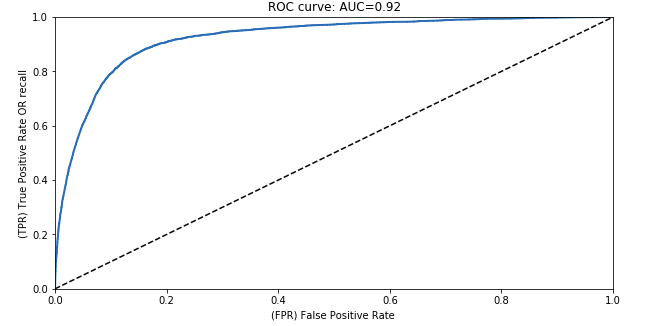
\includegraphics[scale=0.5]{roc}
	\caption{Ejemplo de curva ROC}
	\label{fig:roc}
\end{figure}
Lo ideal, es que la gráfica se acerque a la esquina superior izquierda lo máximo posible, ya que implicaría que se esta clasificando como correctos todas las muestras positivas y ninguna muestra negativa se está clasificando como positiva.\\
Se puede usar el área bajo la curva como una métrica para comprobar como de bueno es el modelo. Esta métrica se conoce como \textbf{AUC} (Area Under Curve).\\
En la Figura \ref{fig:roc} se puede observar una curva ROC obtenida por un modelo que tuvo un rendimiento muy bueno. Se puede observar que el \textbf{ratio de verdaderos positivos} muy alto cuando el ratio de falsos positivos es bajo. La diagonal que aparece representa el rendimiento que tendría un clasificador aleatorio.
\linebreak